\documentclass[11pt,a4paper]{article}
\newcommand{\intestazione}{Trimero ad anello --- 2. VQE}
% =====================================================================
%  Preambolo comune ai documenti sul dimero (serie "che cosa abbiamo fatto")
%  Incluso con % =====================================================================
%  Preambolo comune ai documenti sul dimero (serie "che cosa abbiamo fatto")
%  Incluso con % =====================================================================
%  Preambolo comune ai documenti sul dimero (serie "che cosa abbiamo fatto")
%  Incluso con \input{preambolo_dimero} subito dopo \documentclass.
% =====================================================================
\usepackage[T1]{fontenc}
\usepackage[utf8]{inputenc}
\usepackage[main=italian,provide=*]{babel}
\usepackage{amsmath,amssymb,mathtools}
\usepackage{graphicx}
\usepackage{booktabs}
\usepackage{colortbl}
\usepackage{xcolor}
\usepackage{geometry}
\usepackage{placeins}
\usepackage{caption}
\usepackage{enumitem}
\usepackage{fancyhdr}
\usepackage{needspace}
\usepackage{tikz}
\usetikzlibrary{arrows.meta,positioning,shapes.geometric,calc,fit,backgrounds}
\usepackage{hyperref}
\hypersetup{colorlinks=true,linkcolor=blu,citecolor=blu,urlcolor=blu}

\geometry{margin=2.5cm}

% --- colori coerenti con quelli delle figure (palette Okabe-Ito)
\definecolor{blu}{HTML}{0072B2}
\definecolor{arancio}{HTML}{E69F00}
\definecolor{verdes}{HTML}{009E73}
\definecolor{rossos}{HTML}{D55E00}
\definecolor{violas}{HTML}{CC79A7}
\definecolor{grigetto}{HTML}{E8E8E8}

\captionsetup{font=small,labelfont=bf,width=0.92\textwidth}

\pagestyle{fancy}
\fancyhf{}
\fancyhead[L]{\small\itshape\intestazione}
\fancyhead[R]{\small\thepage}
\renewcommand{\headrulewidth}{0.3pt}

% --- notazione
\newcommand{\ket}[1]{\lvert #1\rangle}
\newcommand{\bra}[1]{\langle #1 \rvert}
\newcommand{\media}[1]{\langle #1 \rangle}
\newcommand{\vs}[1]{\mathbf{s}_{#1}}

% --- riquadro "in una riga": il messaggio da portare a casa
\newcommand{\messaggio}[1]{%
  \begin{center}
  \begin{minipage}{0.93\textwidth}
  \setlength{\fboxsep}{9pt}%
  \colorbox{grigetto}{\begin{minipage}{\dimexpr\textwidth-2\fboxsep}
  \small\textbf{In una riga.}\enspace #1
  \end{minipage}}
  \end{minipage}
  \end{center}
}

% --- riquadro "come lo sappiamo": la verifica numerica dietro un'affermazione
\newcommand{\verifica}[1]{%
  \begin{center}
  \begin{minipage}{0.93\textwidth}
  \small\textcolor{verdes}{\rule{2.2em}{1.1pt}}\enspace
  \textcolor{verdes}{\textbf{Come lo sappiamo.}}\enspace #1
  \end{minipage}
  \end{center}
  \medskip
}
 subito dopo \documentclass.
% =====================================================================
\usepackage[T1]{fontenc}
\usepackage[utf8]{inputenc}
\usepackage[main=italian,provide=*]{babel}
\usepackage{amsmath,amssymb,mathtools}
\usepackage{graphicx}
\usepackage{booktabs}
\usepackage{colortbl}
\usepackage{xcolor}
\usepackage{geometry}
\usepackage{placeins}
\usepackage{caption}
\usepackage{enumitem}
\usepackage{fancyhdr}
\usepackage{needspace}
\usepackage{tikz}
\usetikzlibrary{arrows.meta,positioning,shapes.geometric,calc,fit,backgrounds}
\usepackage{hyperref}
\hypersetup{colorlinks=true,linkcolor=blu,citecolor=blu,urlcolor=blu}

\geometry{margin=2.5cm}

% --- colori coerenti con quelli delle figure (palette Okabe-Ito)
\definecolor{blu}{HTML}{0072B2}
\definecolor{arancio}{HTML}{E69F00}
\definecolor{verdes}{HTML}{009E73}
\definecolor{rossos}{HTML}{D55E00}
\definecolor{violas}{HTML}{CC79A7}
\definecolor{grigetto}{HTML}{E8E8E8}

\captionsetup{font=small,labelfont=bf,width=0.92\textwidth}

\pagestyle{fancy}
\fancyhf{}
\fancyhead[L]{\small\itshape\intestazione}
\fancyhead[R]{\small\thepage}
\renewcommand{\headrulewidth}{0.3pt}

% --- notazione
\newcommand{\ket}[1]{\lvert #1\rangle}
\newcommand{\bra}[1]{\langle #1 \rvert}
\newcommand{\media}[1]{\langle #1 \rangle}
\newcommand{\vs}[1]{\mathbf{s}_{#1}}

% --- riquadro "in una riga": il messaggio da portare a casa
\newcommand{\messaggio}[1]{%
  \begin{center}
  \begin{minipage}{0.93\textwidth}
  \setlength{\fboxsep}{9pt}%
  \colorbox{grigetto}{\begin{minipage}{\dimexpr\textwidth-2\fboxsep}
  \small\textbf{In una riga.}\enspace #1
  \end{minipage}}
  \end{minipage}
  \end{center}
}

% --- riquadro "come lo sappiamo": la verifica numerica dietro un'affermazione
\newcommand{\verifica}[1]{%
  \begin{center}
  \begin{minipage}{0.93\textwidth}
  \small\textcolor{verdes}{\rule{2.2em}{1.1pt}}\enspace
  \textcolor{verdes}{\textbf{Come lo sappiamo.}}\enspace #1
  \end{minipage}
  \end{center}
  \medskip
}
 subito dopo \documentclass.
% =====================================================================
\usepackage[T1]{fontenc}
\usepackage[utf8]{inputenc}
\usepackage[main=italian,provide=*]{babel}
\usepackage{amsmath,amssymb,mathtools}
\usepackage{graphicx}
\usepackage{booktabs}
\usepackage{colortbl}
\usepackage{xcolor}
\usepackage{geometry}
\usepackage{placeins}
\usepackage{caption}
\usepackage{enumitem}
\usepackage{fancyhdr}
\usepackage{needspace}
\usepackage{tikz}
\usetikzlibrary{arrows.meta,positioning,shapes.geometric,calc,fit,backgrounds}
\usepackage{hyperref}
\hypersetup{colorlinks=true,linkcolor=blu,citecolor=blu,urlcolor=blu}

\geometry{margin=2.5cm}

% --- colori coerenti con quelli delle figure (palette Okabe-Ito)
\definecolor{blu}{HTML}{0072B2}
\definecolor{arancio}{HTML}{E69F00}
\definecolor{verdes}{HTML}{009E73}
\definecolor{rossos}{HTML}{D55E00}
\definecolor{violas}{HTML}{CC79A7}
\definecolor{grigetto}{HTML}{E8E8E8}

\captionsetup{font=small,labelfont=bf,width=0.92\textwidth}

\pagestyle{fancy}
\fancyhf{}
\fancyhead[L]{\small\itshape\intestazione}
\fancyhead[R]{\small\thepage}
\renewcommand{\headrulewidth}{0.3pt}

% --- notazione
\newcommand{\ket}[1]{\lvert #1\rangle}
\newcommand{\bra}[1]{\langle #1 \rvert}
\newcommand{\media}[1]{\langle #1 \rangle}
\newcommand{\vs}[1]{\mathbf{s}_{#1}}

% --- riquadro "in una riga": il messaggio da portare a casa
\newcommand{\messaggio}[1]{%
  \begin{center}
  \begin{minipage}{0.93\textwidth}
  \setlength{\fboxsep}{9pt}%
  \colorbox{grigetto}{\begin{minipage}{\dimexpr\textwidth-2\fboxsep}
  \small\textbf{In una riga.}\enspace #1
  \end{minipage}}
  \end{minipage}
  \end{center}
}

% --- riquadro "come lo sappiamo": la verifica numerica dietro un'affermazione
\newcommand{\verifica}[1]{%
  \begin{center}
  \begin{minipage}{0.93\textwidth}
  \small\textcolor{verdes}{\rule{2.2em}{1.1pt}}\enspace
  \textcolor{verdes}{\textbf{Come lo sappiamo.}}\enspace #1
  \end{minipage}
  \end{center}
  \medskip
}


\title{\bfseries Trovare lo stato fondamentale con un circuito\\[2pt]
\large Documento 2 --- VQE, e perché qui RBS non basta dove sul dimero bastava}
\author{Samuele Schiavi \\ \small Tesi triennale in Fisica, Università di Parma
--- Relatore: Prof.\ Alessandro Chiesa}
\date{}

\begin{document}
\maketitle
\thispagestyle{fancy}

\section{Stesso principio, stesso strumento diagnostico}

Il VQE cerca $\boldsymbol\theta^*=\arg\min_{\boldsymbol\theta}
\bra{\psi(\boldsymbol\theta)}H\ket{\psi(\boldsymbol\theta)}$, come sul
dimero. Qui l'energia esatta è nota (Documento 1), quindi il VQE resta uno
strumento diagnostico: misura quanto bene un dato circuito rappresenta lo
stato giusto, tramite la fidelity $\mathcal F=|\langle\psi_{\rm
VQE}|\psi_0\rangle|^2$ (convenzione al quadrato, quella usata in tutto
questo pacchetto).

\medskip
\noindent\textbf{Esatto.} $\ket{\psi_0}$, da \texttt{np.linalg.eigh}.
\noindent\textbf{Vero.} $\ket{\psi_{\rm VQE}}=\ket{\psi(\boldsymbol\theta^*)}$,
circuito eseguito genuinamente (\texttt{Statevector}), mai una scorciatoia.

\section{Due famiglie di blocco $M$-conservante}

Stessa struttura esterna per entrambe: una $X$ sul qubit $0$, poi un blocco
per ciascuno dei tre legami $(1,2),(2,3),(3,1)$ --- tre parametri --- poi tre
rotazioni $R_y$ indipendenti, una per qubit --- altri tre parametri. Sei
parametri in tutto, per entrambe le famiglie: cambia solo il blocco a due
qubit usato sui legami.

\begin{figure}[htbp]
\centering
\begin{minipage}{0.47\textwidth}
\centering
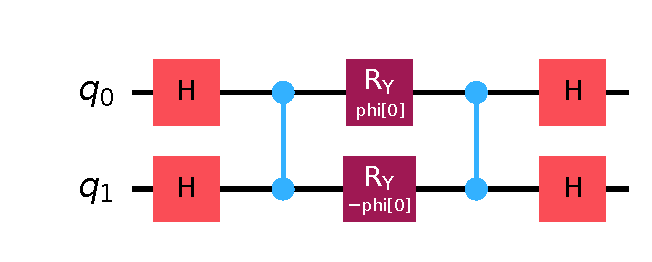
\includegraphics[width=0.85\textwidth]{figure/circ_rbs_espanso_anello}
\\ \textbf{RBS$(\varphi)$}
\end{minipage}
\hfill
\begin{minipage}{0.47\textwidth}
\centering
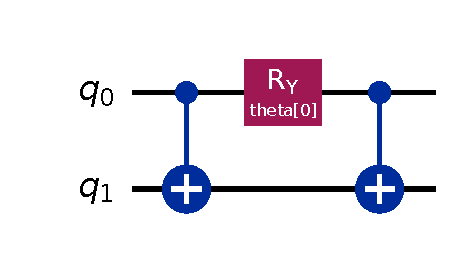
\includegraphics[width=0.85\textwidth]{figure/circ_w_espanso_anello}
\\ \textbf{$W(\theta)$}
\end{minipage}
\caption{I due blocchi a confronto, stessa definizione già validata sul
dimero. RBS: due CZ attorno a una coppia $R_y(\varphi),R_y(-\varphi)$,
sandwiched fra Hadamard --- una rotazione di Givens reale, con un
\textbf{solo} parametro libero $\varphi$ nonostante i due gate $R_y$: il
secondo usa $-\varphi$, lo stesso angolo con segno cambiato, non un
angolo indipendente. $W$: due CNOT attorno a un'unica $R_y(\theta)$ ---
lo stesso blocco che sul dimero era chiamato ``ansatz base''; qui,
riusando il nome della famiglia canonica di Crippa et al., si chiama $W$.}
\label{fig:blocchi}
\end{figure}
\FloatBarrier

\subsection*{Le due forme complete, compatta ed estesa}

\begin{figure}[htbp]
\centering
\begin{minipage}{0.48\textwidth}
\centering
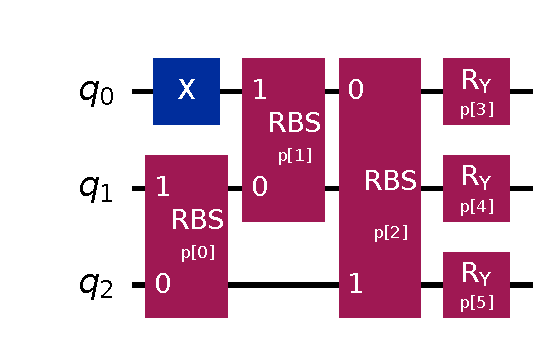
\includegraphics[width=\textwidth]{figure/circ_rbs2q_anello}
\\ RBS-2q.6 (compatta)
\end{minipage}
\hfill
\begin{minipage}{0.48\textwidth}
\centering
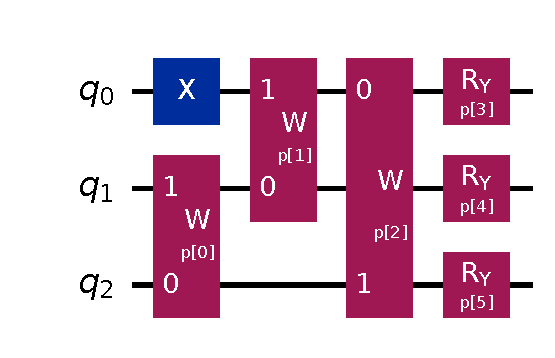
\includegraphics[width=\textwidth]{figure/circ_w2q_anello}
\\ $W$-2q.6 (compatta)
\end{minipage}
\caption{L'ansatz completo, forma compatta (blocchi come scatole nere):
$X$ sul qubit 0, tre blocchi sui tre legami, tre rotazioni $R_y$ finali
indipendenti. Stessa struttura esterna per entrambe le famiglie, cambia
solo il blocco a due qubit.}
\label{fig:ansatz-completo}
\end{figure}
\FloatBarrier

\begin{figure}[htbp]
\centering
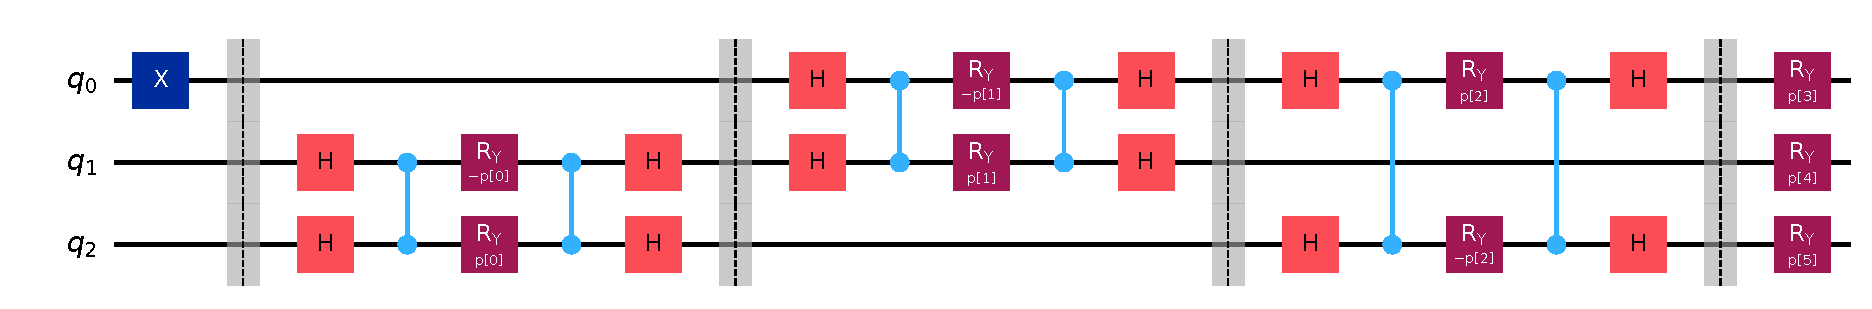
\includegraphics[width=\textwidth]{figure/circ_rbs2q_anello_espanso}
\\[4pt]
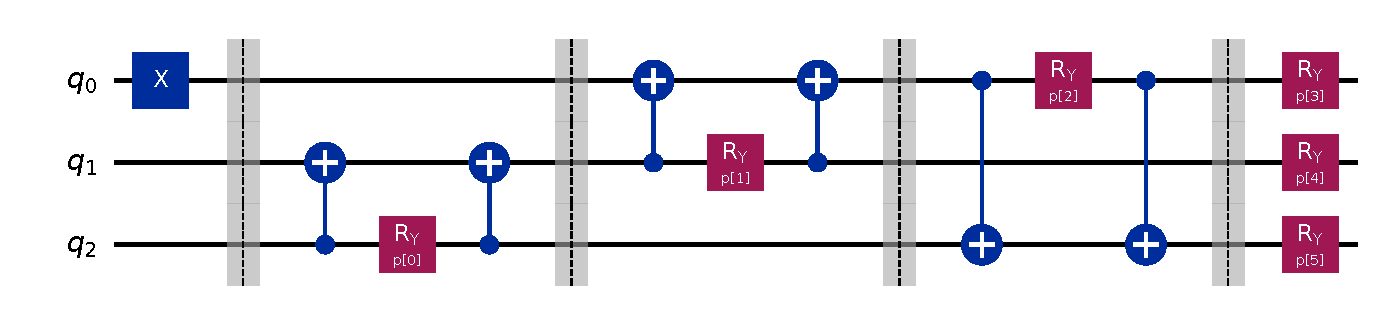
\includegraphics[width=\textwidth]{figure/circ_w2q_anello_espanso}
\caption{Le stesse due forme, completamente espanse in gate elementari
(nessuna scatola). \textbf{Sopra}: RBS-2q.6 --- Hadamard, CZ, $R_y$ ripetuti
per ciascuno dei tre blocchi. \textbf{Sotto}: $W$-2q.6 --- CNOT, $R_y$,
CNOT per ciascun blocco, visibilmente più corto. Stesso numero di CNOT
(6) in entrambe, ma RBS-2q.6 usa quasi il doppio dei gate a un qubit
(confermato nel conteggio dopo transpilazione, Documento 2 §``Come lo
sappiamo'').}
\label{fig:ansatz-completo-espanso}
\end{figure}
\FloatBarrier
\FloatBarrier

\section{A campo critico, senza DM: le due famiglie sono equivalenti}

Al punto critico $b_c/J=2.4$, $D=0$: entrambe le famiglie, con i sei
parametri completi, raggiungono $\mathcal F=1.000000$ (verificato a sei
cifre, multistart con seme). Nessuna sorpresa qui --- è il caso facile,
analogo al pannello sinistro del dimero.

\section{Sotto DM: qui il confronto ha un esito diverso da quello del dimero}
\label{sec:rbs-vs-w}

Al punto di lavoro \textbf{Scenario A} ($b/J=b_c=2.4$, $D/J=0.15$, Opzione
B): multistart con ottimizzazione diretta della fidelity, venti punti di
partenza casuali.

\begin{table}[htbp]
\centering
\small
\renewcommand{\arraystretch}{1.3}
\begin{tabular}{@{}lcc@{}}
\toprule
\rowcolor{grigetto}
\textbf{Ansatz} & \textbf{fidelity} & $1-\mathcal F$ \\
\midrule
RBS-2q (6 par.) & $0.9999110739$ & $8.89\times10^{-5}$ \\
$W$-2q.6 (6 par.) & $0.9999999999999996$ & $\approx4\times10^{-16}$ \\
\bottomrule
\end{tabular}
\caption{Fidelity sotto DM (Scenario A), stessa struttura di circuito, stesso
numero di parametri, differiscono solo nel blocco a due qubit. RBS ha un
tetto reale, piccolo ma non nullo; $W$ raggiunge l'esatto a precisione
macchina.}
\label{tab:rbs-vs-w}
\end{table}
\FloatBarrier

Questo è \textbf{l'opposto} di quanto succede sul dimero, dove RBS (più
economico in gate) è la scelta raccomandata e $W$ (la famiglia originale di
Crippa et al.) è più costosa senza vantaggi. Qui RBS ha un tetto
strutturale vero, per quanto piccolo, e $W$ no.

\verifica{Il costo in gate non spiega la differenza --- è comparabile.
Transpilato in base $\{rz,sx,x,cx\}$, livello di ottimizzazione 3: entrambe
le famiglie usano $6$ CNOT (due per blocco, tre blocchi). $W$-2q.6 usa
$25$ gate a un qubit ($13$ sx $+12$ rz); RBS-2q ne usa $46$ ($25$ rz$+21$
sx) --- quasi il doppio, per via delle Hadamard e delle due $R_y$ per
blocco di RBS contro l'unica $R_y$ di $W$. $W$ costa meno, non di più, e
allo stesso tempo ottiene fidelity migliore: nessun compromesso da
giustificare.}

\begin{figure}[htbp]
\centering
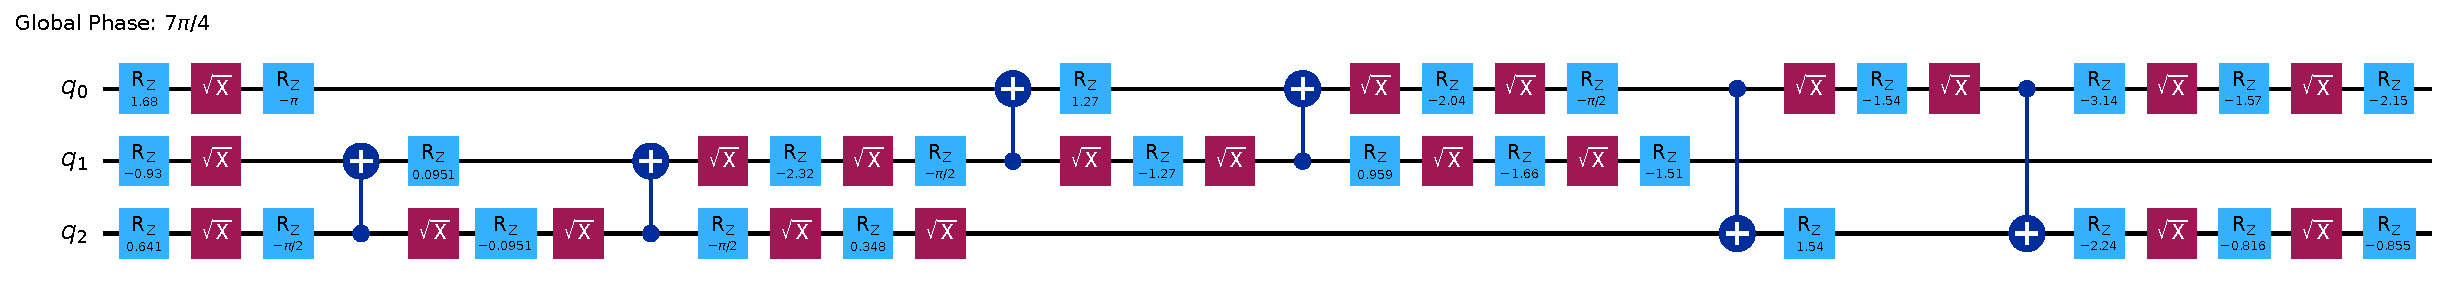
\includegraphics[width=\textwidth]{figure/circ_rbs2q_anello_compilato}
\\[6pt]
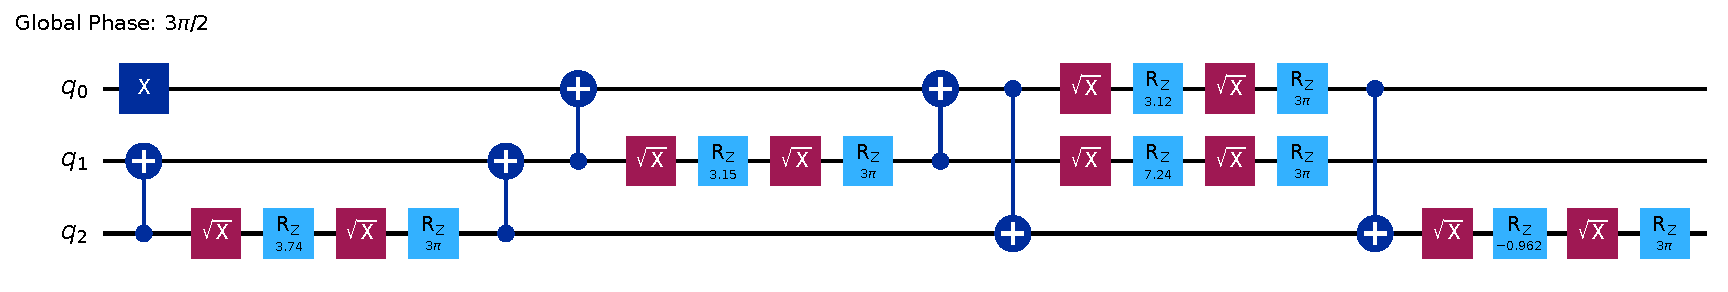
\includegraphics[width=\textwidth]{figure/circ_w2q_anello_compilato}
\caption{I due ansatz compilati in base $\{rz,\text{sx},x,cx\}$
(``sx'' è $\sqrt{X}$, la radice quadrata di $X$), ai rispettivi parametri
ottimali a Scenario A. \textbf{Sopra}: RBS-2q.6. \textbf{Sotto}: $W$-2q.6,
visibilmente più corto. Conteggio qui leggermente diverso da quello sopra
(calcolato su assegnazioni casuali): ai valori ottimali di $W$-2q.6 tre
angoli sono vicini a zero ($p_1{\approx}0.012$, $p_2{\approx}{-}0.024$,
$p_3{\approx}0$), e il compilatore semplifica di conseguenza --- stesso
fenomeno di non invarianza del conteggio gate rispetto ai parametri già
noto altrove nel progetto, non un errore.}
\end{figure}
\FloatBarrier

\subsection*{Perché: il peso fuori dal settore, non un limite di parametri}

Il blocco RBS puro (senza le tre $R_y$ finali che rompono la conservazione
di $M$) resta confinato nel settore a cui appartiene lo stato di partenza
$X\ket{000}=\ket{100}$ --- magnetizzazione $M=+1/2$, Hamming weight $1$.
Verificato direttamente: il peso della vera GS a Scenario A in quel settore
è $0.00098$, e la fidelity massima raggiungibile da un ansatz confinato lì
--- qualunque il numero di blocchi RBS, ripetuti quante volte si vuole ---
coincide con quel peso a sette cifre:

\begin{table}[htbp]
\centering
\small
\renewcommand{\arraystretch}{1.3}
\begin{tabular}{@{}ccc@{}}
\toprule
\rowcolor{grigetto}
\textbf{giri di blocchi RBS (puro, senza $R_y$)} & \textbf{parametri} & \textbf{fidelity} \\
\midrule
1 & 3 & $0.0009814687$ \\
2 & 6 & $0.0009814687$ \\
3 & 9 & $0.0009814687$ \\
\bottomrule
\end{tabular}
\caption{Il tetto non si sposta aggiungendo giri --- stesso principio già
visto sul dimero (Tab.~4 del Documento 2 gemello): ripetere un blocco
confinato allo stesso settore non aggiunge direzioni raggiungibili. Il
valore coincide, a sette cifre, con il peso della vera GS nel settore
$M=+1/2$ ($0.00098$) --- non è un limite numerico dell'ottimizzatore, è
geometria: la fidelity massima di uno stato confinato in un sottospazio è
il peso della proiezione della GS su quel sottospazio.}
\label{tab:tetto-anello}
\end{table}
\FloatBarrier

A differenza del dimero, dove aggiungere due rotazioni $R_y$ indipendenti
dopo un solo blocco RBS già riparava completamente il problema
($\mathcal F=1$), qui \textbf{le tre $R_y$ finali non bastano a chiudere
del tutto il tetto}: RBS-2q a sei parametri (con $R_y$) resta a
$0.99991$, non $1$. Verificato che aggiungere un secondo giro completo di
blocchi RBS (sei parametri sui legami, più le tre $R_y$ finali, nove in
tutto) \textbf{non sposta il risultato}: fidelity identica,
$0.9999110739$, a dieci cifre. Il tetto di RBS su questo sistema, con
questa preparazione iniziale, è più ostinato che sul dimero.

\messaggio{Sul dimero, rompere la conservazione di $M$ con due rotazioni
locali bastava a raggiungere qualunque stato. Sul trimero, romperla con
tre rotazioni locali aiuta molto (da $F\approx0.001$ a $F\approx0.9999$)
ma non chiude l'ultimo tratto. $W$, con lo stesso numero di parametri e
meno gate, lo chiude per intero. La differenza fra le due famiglie non è
quindi solo un fatto di efficienza in gate, come sul dimero: qui è anche
una differenza di potere espressivo, a parità di parametri.}

\section{Ansatz canonico: $W$-2q.6}

Per il resto di questa serie (Documenti 3 e 4) e per la pipeline di rumore
(pacchetto separato), l'ansatz usato è \textbf{$W$-2q.6}: sei parametri, la
Fig.~\ref{fig:ansatz-completo}, fidelity esatta a precisione macchina al
punto Scenario A.

\begin{table}[htbp]
\centering
\small
\renewcommand{\arraystretch}{1.3}
\begin{tabular}{@{}lc@{}}
\toprule
\rowcolor{grigetto}
\textbf{Quantità} & \textbf{valore} \\
\midrule
$E_\text{VQE}$ & $-5.53437001739340$ \\
$E_\text{esatto}$ & $-5.53437001739350$ \\
$\Delta E$ & $9.8\times10^{-14}$ \\
$\mathcal F$ & $0.99999999999961$ \\
\bottomrule
\end{tabular}
\caption{Risultato dell'ansatz canonico $W$-2q.6 a Scenario A, multistart a
12 punti di partenza casuali: tutti e 12
convergono allo stesso ottimo.}
\end{table}
\FloatBarrier

\section{Uno sweep in campo: verificato, nessun ramo necessario}

Verificato su tredici valori di $b/J$ fra $0.3$ e $4.5$, DM Opzione B
acceso ($D/J=0.15$) --- inclusi punti ben sotto e ben sopra l'incrocio, e
il punto dell'incrocio stesso ($b/J=2.372$): nessuna logica a rami
necessaria per l'ansatz $W$-2q.6, a differenza dell'ansatz minimo del
dimero.

\begin{table}[htbp]
\centering
\small
\renewcommand{\arraystretch}{1.2}
\begin{tabular}{@{}ccccccc@{}}
\toprule
\rowcolor{grigetto}
$b/J$ & $0.3$ & $0.8$ & $1.2$ & $1.8$ & $2.372$ (incrocio) & $3.0$ \\
\midrule
$\mathcal F$ & $1.0$ & $1.0$ & $1.0$ & $1.0$ & $1.0$ & $1.0$ \\
\bottomrule
\end{tabular}
\caption{Fidelity dell'ansatz $W$-2q.6 (nessun ramo, stesso $X\ket{000}$
di partenza ovunque), campionata su tredici punti fra $b/J=0.3$ e
$b/J=4.5$: $\mathcal F=1.00000000$ su \textbf{tutti} i punti testati,
incluso quello immediatamente all'incrocio.}
\end{table}
\FloatBarrier

\bigskip
\noindent\footnotesize\textit{Riferimento.} Per il modello e la famiglia di
ansatz $W_{ij}(\theta)$ di riferimento: A.~Crippa et al., \emph{Simulating
Static and Dynamic Properties of Magnetic Molecules with Prototype Quantum
Computers}, Magnetochemistry \textbf{7}, 117 (2021).

\end{document}
